\section{\label{sec:nmp:analysis}Asynchronous system analysis}

This \namecref{sec:nmp:analysis} examines and analyses the asynchronous \gls{pe}-specific system of \cref{sec:nmp:pespecific}.  Firstly, it describes and proves several properties about the system, in particular, that the asynchronous system exchanges precisely the same number of \gls{nm} messages as the \gls{gs} system of \cref{sec:nmp:systemwide}.  Then, it states three conjectures about the system, yet to be proven or disproven mathematically, before examining the asynchronous system's complexity from the standpoint of the rules and symbols used.  Lastly, the \namecref{sec:nmp:analysis} discusses some visualisations of the propagation of ``influence'' from one \gls{pe} in a \gls{fne} grid to others, over multiple steps.

Recall that the fundamental difference between in behaviour between the \gls{gs}, \gls{ls} and asynchronous variants is the timing of when they send out new messages relating to when they have received messages for the previous generation.  Under the \gls{gs} approach, \emph{every} \gls{pe} waits until every other \gls{pe} has received all incoming messages before progressing.  Following the \gls{ls} methodology, each \gls{pe} waits until it has received all of its due incoming messages before proceeding, \emph{but without regard} to any other \gls{pe}.  Lastly, for the asynchronous variant, a \gls{pe} waits only until it has received the \(n - 1\) required messages from the other neighbours of generation \(g\) before sending the appropriate generation \(g + 1\) message to the \(n^\text{th}\) neighbour.

\subsection{\label{sec:nmp:msgprops}Messaging properties and behaviours}

Consider a cell (\gls{pe}) $\pi_0$ in the asynchronous framework of \cref{sec:nmp:pespecific},
where the maximum generation count is $I$, set by the environment via $\cpfunc{i}{I}$.
Without loss of generality, 
we consider only a \gls{fne} system and
assume that $\pi_0$ is a non-border/non-corner cell with four neighbours, 
$\pi_k$, accessible via channels labelled by $k \in \{ 1, 2, 3, 4 \}$. 

\begin{lemma}\label{lemma:nmp:-0}
    For any $k \in \{ 1, 2, 3, 4 \}$, after each round except the last,
    cell $\pi_0$ contains exactly one $k$-tagged value $\cpvv{k}{\cpdiscard}{\cpdiscard}$, 
    which is accepted from channel $k$ 
    --- except the first round, when that value $v$ comes from the environment channel $e$.
\end{lemma}

\begin{proof}
    By \cpruleref{rule:nmp:proxspec:recvinputs}, cell $\pi_0$ starts by accepting a value $\cpvv{k}{0}{\cpdiscard}$, from the environment channel $e$.
    \cpRuleref{rule:nmp:proxspec:recvfromneighs} gives the only possibility of obtaining another $k$-tagged value, by replacing the current value $v$ with another value $v'$, accepted from channel $k$.
\end{proof}

\begin{remark}
    In fact, \cref{lemma:nmp:-0} holds practically at all times, not just at the end of each round.  The only exceptions are: before the start of the system's evolution and application of \cpruleref{rule:nmp:proxspec:recvinputs}; and after the start of the finalisation phase, specifically after applying \cpruleref{rule:nmp:proxspec:finaloracle}.
\end{remark}

\begin{lemma}\label{lemma:nmp:-1}
    For any $k \in \{ 1, 2, 3, 4 \}$, the time sequence of generation numbers $g \geq 0$ of accepted values $\cpvv{k}{g}{\cpdiscard}$ forms an arithmetic progression with step size one.
\end{lemma}

\begin{proof}
    Proof by induction. Cell $\pi_0$ starts with value $\cpvv{k}{0}{\cpdiscard}$, received via the environment channel $e$.
    Assume that this hypothesis holds for a given $g \geq 0$, appearing as a generation number in value $\cpvv{k}{g}{\cpdiscard}$. \cpRuleref{rule:nmp:proxspec:recvfromneighs} gives the only possibility of changing this number, by replacing the current value with another $v$ value, where the generation number is strictly greater by one, 
    $\cpvv{k}{g+1}{\cpdiscard}$.
\end{proof}

\begin{remark}\label{remark:nmp:-1}
The conclusion of \cref{lemma:nmp:-1} will hold even in the hypothetical case that cell $\pi_k$ would be allowed to send multiple copies of the same message $v$. 
Only the first received copy will be accepted, and the rest will be ignored,
courtesy of \cpruleref{rule:nmp:proxspec:recvfromneighs}. However, this is not the case, as excess \(w\) \gls{oq} messages are deleted by \cpruleref{rule:nmp:proxspec:uniq}. 
\end{remark}

\begin{lemma}\label{lemma:nmp:-2}
    For any $k \in \{ 1, 2, 3, 4 \}$, if channels are reliable and cell $\pi_k$ sends a sequence of messages that reach $\pi_0$ as $\cpvv{k}{g}{\cpdiscard}$, $g \in [1,I]$, 
    then $\pi_0$ accepts all these values in the order of their increasing generation numbers.
\end{lemma}

\begin{proof}
    Channels are reliable, so no message is lost. Channels in \gls{cps} are not inherently FIFO, but cell $\pi_0$ will still pick messages with increasing generation numbers, by \cref{lemma:nmp:-1}.
    As defined by the async version of the model, any messages arriving out-of-order are not lost, but stored in a multiset at the end of the channel
    and will be picked when their time comes.
\end{proof}

\begin{lemma}\label{lemma:nmp:-3}
    For any $k \in \{ 1, 2, 3, 4 \}$, and $g \in [1, I]$: cell $\pi_0$ sends one generation $g$ value $v$ over channel $k$, if and only if $\pi_0$ has received three generation $g-1$ values $v$ from three distinct channels $k' \in 
    \{ 1, 2, 3, 4 \} \setminus \{ k \}$.
\end{lemma}

\begin{proof}
    \textbf{Only if}. Assume that $\pi_0$ sends out a generation $g$ message $v$ over channel $k$.   
    This may only happen by \cpruleref{rule:nmp:proxspec:recvfromoracle}, where $\pi_0$ just forwards the same message $v$, received as $w$ from its oracle. 
    \cpRuleref{rule:nmp:proxspec:sendtooracle} triggers the oracle to build this message $w$, based on three other $v$ messages 
    $\cpvv{k_1}{g_1}{d_1}$, $\cpvv{k_2}{g_2}{d_2}$, $\cpvv{k_3}{g_3}{d_3}$, 
    where $g_1 = g-1$, $g_2, g_3 \geq g_1$, and $k, k_1, k_2, k_3$ are all distinct.
    By \cref{lemma:nmp:-2}, $\pi_0$ must have also received two generation $g-1$ values $v$, from $k_2$ and $k_3$.
    Thus, cell $\pi_0$ has received three values $\cpvv{k_1}{g-1}{d_1}$, $\cpvv{k_2}{g-1}{\cpdiscard}$, $\cpvv{k_3}{g-1}{\cpdiscard}$.
    
    \textbf{If}. Assume that $\pi_0$ accepts three values $\cpvv{k_1}{g'}{d_1}$, $\cpvv{k_2}{g'}{\cpdiscard}$, $\cpvv{k_3}{g'}{\cpdiscard}$, where $g' = g - 1 \geq 0$. These values need not arrive at the same round. Without loss of generality, assume that $\pi_0$ has just received the first value, $\cpvv{k_1}{g'}{d_1}$, while the other values may have been received and even updated already, 
    $\cpvv{k_2}{g'+h_2}{d_2}$, $\cpvv{k_3}{g'+h_3}{d_3}$, $h_2, h_3 \geq 0$.
    \cpRuleref{rule:nmp:proxspec:makews} applies and creates at least two identical \(w\) messages $\cpvw{k_4}{g' + 1}{d}$, where \(d = \cpfunc{d}{d_1}, \, \cpfunc{d}{d_2}, \, \cpfunc{d}{d_3}\). Additional $w$ messages may be created, if either $h_2=0$, or $h_3=0$, or both. This doesn't matter, 
    as excess \(w\) messages are deleted by \cpruleref{rule:nmp:proxspec:uniq}, so only one $\cpvw{k_4}{g' + 1}{d}$ remains.
    This message goes to the oracle, 
    which creates and returns the value $\cpvw{k_4}{g'+1}{d'} = \cpvv{k_4}{g}{d'}$, 
    further forwarded by \cpruleref{rule:nmp:proxspec:recvfromoracle} to $\pi_{k_4}$, over channel $k_4$.
\end{proof}

\begin{remark}
    The behaviour of Lemma~\ref{lemma:nmp:-3} is also true for the \gls{gs} and \gls{ls} variants too.  The key difference for the asynchronous variant is that the new outgoing message for generation \(g\) is sent as soon as possible after those three messages for generation \(g - 1\) have been received, whereas the other two variants will await receipt of the final also message before sending any new ones.
\end{remark}

\begin{theorem}\label{theorem:nmp:-1}
    For each $k \in \{ 1, 2, 3, 4 \}$, and each $g \in [0, I]$:
    \begin{inparaenum}[(i)]
        \item\label{enumitem:nmp:analysis:-1:1} $\pi_0$ receives one $k$-tagged generation $g$ value $v$; and
        \item\label{enumitem:nmp:analysis:-1:2} if $g < I$, $\pi_0$ sends one $k$-tagged generation $g+1$ value $v$.
    \end{inparaenum}
\end{theorem}

\begin{proof}
By bounded induction on $g$. Base case: $g = 0$. By \cpruleref{rule:nmp:proxspec:recvinputs}, cell $\pi_0$ receives \emph{four} $k$-tagged generation $g$ values -- one for each $k \in \{ 1, 2, 3, 4 \}$ -- from the environment channel $e$ (acting on behalf of its neighbour channels). By \cref{lemma:nmp:-3}, applied \emph{four} times, $\pi_0$ sends out \emph{four} generation $g+1$ values $v$, one over each channel $k$.

Induction step: assume that the induction hypothesis holds for 
$g \in [0, I)$, and we prove that it still holds for $g+1$.
The induction hypothesis holds for all cells, 
including $\pi_0$ and $\pi_k$. 
% Thus, by part (ii), each cell $\pi_k$ sends a generation $g+1$ value $v$,
Thus, by part (\ref{enumitem:nmp:analysis:-1:2}), each cell $\pi_k$ sends a generation $g+1$ value $v$, 
which is further received by $\pi_0$, as $\cpvv{k}{g+1}{\cpdiscard}$.
This proves part (\ref{enumitem:nmp:analysis:-1:1}) of the induction step.

If $g+1 < I$, rule 9 does not apply and, 
as shown by \cref{lemma:nmp:-3}, applied \emph{four} times, 
$\pi_0$ sends out \emph{four} generation $g+2$ values $v$, one over each channel $k$.
This proves part (\ref{enumitem:nmp:analysis:-1:2}) of the hypothesis.
\end{proof}

\begin{theorem}\label{theorem:nmp:-2}
    Cell (\gls{pe}) \(\pi_0\) does not send any message to its neighbours at generation \(g > I\).
\end{theorem}

\begin{proof}
    \Gls{oq} \(w\) messages (and thus indirectly \gls{nm} \(v\) messages) are created only by \cpruleref{rule:nmp:proxspec:makews}, with generation counts \(g + 1\), only if \(g + 1 \leq I\).  The promoter \(\cpfunc{i}{G1\cpdiscard}\) for \cpruleref{rule:nmp:proxspec:makews} prevents the creation of any \(w\) message with a larger generation count.
\end{proof}

\begin{theorem}\label{theorem:nmp:-3}
    For each cell $\pi_0$, the neighbourhood (inter-cell) messaging loop stops after receiving the last generation $I$ value.
\end{theorem}

\begin{proof}
    After receiving the last generation \(I\) message, \cpruleref{rule:nmp:proxspec:makews} does not apply (per \cref{theorem:nmp:-2}), and instead control flows by \cpruleref{rule:nmp:proxspec:skiptorecv} to state \(s_5\), then to \(s_6\) by \cpruleref{rule:nmp:proxspec:clearrs}.  Finally, \cpruleref{rule:nmp:proxspec:movetoend} applies, and the control flow breaks out of the main messaging loop, proceeding to state \(s_7\) and the finalisation phase, where no further \gls{nm} occurs. 
\end{proof}

\begin{theorem}\label{theorem:nmp:-4}
    For the asynchronous system in \cref{sec:nmp:pespecific}, 
    each cell (\gls{pe}) sends and receives the same number of messages as in the \gls{gs} system in \cref{sec:nmp:systemwide} and the \gls{ls} system in \cref{sec:nmp:localsync}.   
    Thus, the system as a whole uses the same number of messages.
\end{theorem}

\begin{proof}
    Direct consequence of \cref{theorem:nmp:-1,theorem:nmp:-3}
\end{proof}

\begin{remark}\label{remark:nmp:-2}
    The evolution of the asynchronous version can be suggestively summarised by
    analysing the following four typical cases of cell $\pi_0$ snapshots,
    which focus on the received values having the \emph{least generation number}, here indicated by $g$.
    Note that each star (*) indicates the channel of the incoming value 
    that triggers the sending of a generation $g+1$ message, 
    \emph{not} the channel over which this is sent.
    Without loss of generality, in the case of confluent non-determinism,
    stars are allocated to the first possible choice (for illustrative purposes).
    
    \begin{enumerate}
    \item $(g?***, g?*, g?, g?)$: 
    $\pi_0$ receives all \emph{four} generation $g$ values in the same round, by \cpruleref{rule:nmp:proxspec:recvfromneighs}. 
    As shown by \cref{lemma:nmp:-3}, applied \emph{four} times, 
    $\pi_0$ sends \emph{four} generation $g+1$ values.
    \cpRuleref{rule:nmp:proxspec:makews} will initially create \emph{six} \gls{oq} messages per neighbour (for a total of 24)
    but the excess ones will be deleted, so exactly one \(w\) message per channel will remain and be sent to the oracle.
    
    \medskip
    \item $(g?***, g?*, g?, g_4)$, $g < g_4$: 
    $\pi_0$ receives \emph{three} generation $g$ values in the same round, by \cpruleref{rule:nmp:proxspec:recvfromneighs}.
    The fourth value is at least one generation ahead.    
    This case evolves similarly to case (1) above, with a few changes in the details.
    As shown by \cref{lemma:nmp:-3}, still applied \emph{four} times, 
    $\pi_0$ sends \emph{four} generation $g+1$ values.
    The rules will create \emph{four} \gls{oq} messages for each of the first three channels,
    and \emph{six} \gls{oq} messages for the last channel (for a total of 18),
    but the excess ones will be deleted, so exactly one \gls{oq} message per channel will remain and be sent.
    
    \medskip
    \item $(g?***, g?*, g_3, g_4)$, $g < g_3, g_4$: 
    $\pi_0$ receives \emph{two} generation $g$ values in the same round, by \cpruleref{rule:nmp:proxspec:recvfromneighs}.
    The other two values are at least one generation ahead.    
    This case evolves similarly to case (2) above, with a few changes in the details.
    As shown by \cref{lemma:nmp:-3}, still applied \emph{four} times, 
    $\pi_0$ sends \emph{four} generation $g+1$ values.
    The rules will create \emph{two} \gls{oq} messages for each of the first two channels,
    and \emph{four} \gls{oq} messages for the last two channels (for a total of 12),
    but the excess ones will be deleted, so only one \gls{oq} message per channel will remain and be sent.
    
    \medskip
    \item $(g?***, g_2, g_3, g_4)$, $g < g_2, g_3, g_4$: 
    $\pi_0$ receives \emph{one} single generation $g$ value in a given round, by \cpruleref{rule:nmp:proxspec:recvfromneighs}.
    The last three values are at least one generation ahead.
    As shown by \cref{lemma:nmp:-3}, applied \emph{three} times, 
    $\pi_0$ sends \emph{three} generation $g+1$ values.
    The rules will create and use \emph{two} \gls{oq} messages for each of the last three channels (for a total of 6), but the excess ones will be deleted.
    
    \medskip
    The question arises: when will $\pi_0$ send its fourth generation $g+1$ value, over channel $1$? Brief answer: that message was already sent,
    before the current round!
    
    \medskip
    % Indeed, Lemmas~\ref{lemma:nmp:-1},\ref{lemma:nmp:-2} show that,
    Indeed, \cref{lemma:nmp:-1,lemma:nmp:-2} show that,
    from each channel $k \in \{ 2, 3, 4\}$, 
    $\pi_0$ has received, in order, 
    messages with generation numbers $g, g+1, \ldots, g_k$.
    Consider the round when $\pi_0$ receives the last such message for generation $g$. Without loss of generality, assume that this was from channel $2$.
    Thus, at that round, the summary snapshot was $(g_1, g?, g'_3, g'_4)$,
    with $g_1 < g \leq g'_3, g'_4$.
    By \cref{lemma:nmp:-3}, \emph{one} generation $g+1$ value was then sent over channel $1$.
    \end{enumerate}    
    
    Note also that, at the outset of cases (1,2,3), no other messages for generation $g+1$ will have been sent yet because too few messages at generation $g$ have been received. 
    These notes may be used to create alternate proofs of our main results.

\end{remark}

\subsection{Generational confluence}
The asynchronous system is \emph{not} (necessarily) confluent.  Messages may be received in such an order that the contents of some messages might not be used in the preparation of new messages, since two messages potentially can be received from one neighbour between receipts from a different neighbour.  Nevertheless, for a \gls{pe} to send a message for generation \(g + 1\) to neighbour \(k\), it must have received messages for \emph{at least} generation \(g\) from all other neighbours.  Therefore, no input data will be `out-of-date'.  This concept is given the name \emph{generational confluence}.

\begin{conjecture}\label{conj:nmp:1}
A \gls{nmp} system following the asynchronous rules of \cref{sec:nmp:pespecific} will be \emph{approximately/generationally} confluent.  Under a wide variety of practical conditions (\eg{} when the base synchronous version is convergent), every evolution of the system will produce a similar result, no matter the specific ordering of the messaging.
\end{conjecture}

\begin{conjecture}\label{conj:nmp:2}
    The asynchronous behaviour, specifically the potential for \glspl{pe} to forgo the use of data from particular messages in favour of newer data, will lead to a final output that is no worse than the synchronous variants' and might result in a `better quality' result, for a particular domain-specific meaning of quality.
\end{conjecture}

Determining the truth or falsity of \cref{conj:nmp:1,conj:nmp:2} is still an open problem requiring further study (but see \cref{sec:nmp:convergence}).  Ideally, one would also clarify and quantify what ``similar'' means in this context.

\begin{proposition}\label{prop:nmp:3}
    No matter the approach to \gls{nmp} employed, the most generations any given \gls{pe} may be ahead of any other \gls{pe} on the lattice depends on their distance from each other, as measured by the smallest number of intermediate \glspl{pe} along any path between the two.
\end{proposition}

The requirement for a \gls{pe} to have received messages from every other neighbour before preparing a message to send to the final neighbour means that, at a certain point, a \gls{pe} transitively depends on its neighbours' neighbours in an ever-expanding radius.  A given \gls{pe} cannot send a new message to neighbour 4 until it has received messages from neighbours 1-3.  In turn, neighbour 4 cannot send messages to any of its other neighbours besides the original \gls{pe} until it has received the next message from the original \gls{pe}.  The same then applies to those neighbours of the original \gls{pe}'s neighbour 4, \etc{}.

This reasoning gives rise to the intuition in \cref{prop:nmp:3}.  If one of the \glspl{pe} stops sending messages but has not yet reached its maximum generation, the neighbouring \glspl{pe} will successively be unable to send further messages themselves, which will ripple across the lattice and eventually prevent farther \glspl{pe} from sending further messages as well.  Until the ripple has progressed across the lattice, however, the more remote \glspl{pe} may still send new messages.  Therefore, in all cases where two \glspl{pe} have a path between them, there is an inter-dependency, albeit in some cases far removed.  As yet, no suitable and convincing formal proof of this idea has been found.

\subsection{Rule and symbol complexity}
Overall, the rule and symbol complexity of the system is relatively low, but given that some elements of any specific \gls{nmp} process are abstracted away (\eg{} the oracle), this is likely an underestimate for a given final implementation.

\subsubsection{Rule complexity}
The total system requires 12 rules.  Two for the initialisation phase, eight for the joint \gls{nm} \& \gls{oq} phases -- only two directly involve interaction with the oracle, but others prepare for said interaction -- and two for the finalisation phase.  The two rules that involve direct interaction with the oracle, rules \cpruleref*{rule:nmp:proxspec:sendtooracle} and \cpruleref*{rule:nmp:proxspec:recvfromoracle}, will normally be replaced with an arbitrary new \gls{ruleset}, however.  Thus, it can be said that there are 10 rules relating to the structure and process for \gls{nmp}, and two stub rules which stand in for a more complex process.

\subsubsection{Symbol complexity}
Across all 12 rules, three atoms, eight functors, and nine states are used.  This gives a total symbol complexity of 20 distinct symbols.  As with the rule complexity, there likely will be more symbols used when the \gls{oq} phase is expanded to encompass a desired computation process.

\subsection{Visualisations}
Sequences of visualisations of the evolution of a sample \gls{fne} system have been created to explore the messaging behaviour of \gls{nmp}.  These sequences reflect the changes on a small grid that result from \gls{nmp} following \cref{sec:nmp:pespecific}'s system.  Each square on the grids represents one \gls{pe}, and the \glspl{pe} are assumed to be connected in the standard \gls{fne} manner.

Each sequence was generated using a script by computing values over the grid at the end of each round of messaging and writing the results out to a standalone .tex file, then compiling the .tex file to produce an output .pdf.  In each case, the grid starts with all zero values, except for the centre \gls{pe}, which starts with a `full-strength' value --- represented by wholly white and completely black squares, respectively.  The value to display at a given grid point for each round was in turn computed by selecting the maximum from among the data stored in the corresponding \gls{pe}.

Each of the sequences uses a different method for computing the values present in a given square, and so depicts a different aspect of the spread of the `influence' of the initial data in the centre \gls{pe}.  The approach used here was effectively the \gls{ls} variant, but the results apply equally to the variants.

\subsubsection{Maximum over messages received and internal datum}
\begin{figure}
    \centering
    \subcaptionbox{Round 0}{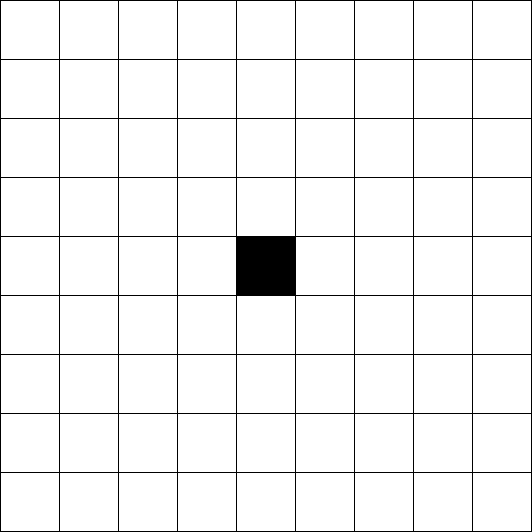
\includegraphics[width=0.19\textwidth]{chapters/nmp/images/grids/maxpdatum/nodelay/maxWithPDatum_no_delays_four_generations_round_0.pdf}}
    \subcaptionbox{Round 1}{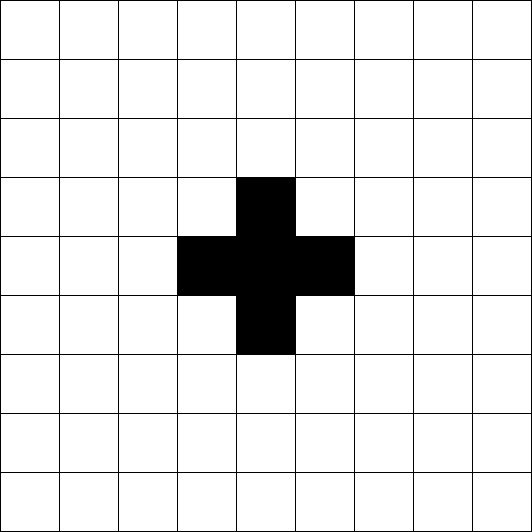
\includegraphics[width=0.19\textwidth]{chapters/nmp/images/grids/maxpdatum/nodelay/maxWithPDatum_no_delays_four_generations_round_1.pdf}}
    \subcaptionbox{Round 2}{
\includegraphics[width=0.19\textwidth]{chapters/nmp/images/grids/maxpdatum/nodelay/maxWithPDatum_no_delays_four_generations_round_2.pdf}}
    \subcaptionbox{Round 3}{
\includegraphics[width=0.19\textwidth]{chapters/nmp/images/grids/maxpdatum/nodelay/maxWithPDatum_no_delays_four_generations_round_3.pdf}}
    \subcaptionbox{Round 4}{
\includegraphics[width=0.19\textwidth]{chapters/nmp/images/grids/maxpdatum/nodelay/maxWithPDatum_no_delays_four_generations_round_4.pdf}}
    \caption[Visualisation of the spread of `influence' from the centre \glsxtrshort{pe} during \glsxtrlong{nmp}]{Visualisation of the spread of `influence' from the centre \gls{pe} during \gls{nmp}.  Each square's value was computed as the maximum over both the last messages received, and a datum stored by the \gls{pe}}
    \label{fig:nmp:maxpdatum}
\end{figure}

The sequence in \cref{fig:nmp:maxpdatum} was produced by using the maximum of the \gls{pe}'s current messages received from the other neighbours \emph{and} a separate value stored internally and updated when computing the new outgoing messages.  The extra value was updated at each step to be the maximum of itself or the messages currently held.  The net effect of this was to ensure that when a message carrying information from the centre \gls{pe} arrived, the current \gls{pe} would turn black and remain that way.  \Cref{fig:nmp:maxpdatum} shows that this information propagates outwards as expected, given the nature of the updates.

\begin{figure}
    \centering
    \subcaptionbox{Round 0}{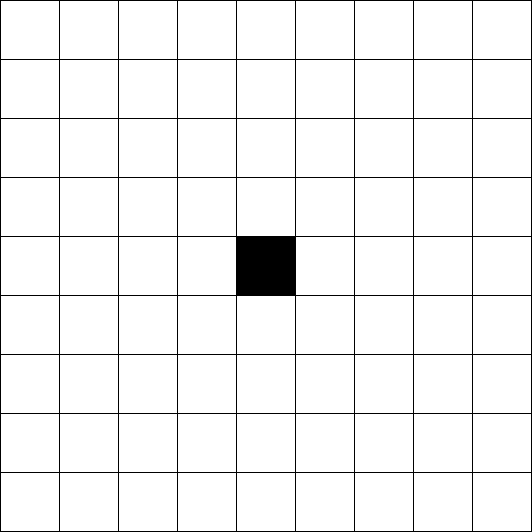
\includegraphics[width=0.19\textwidth]{chapters/nmp/images/grids/maxpdatum/delay2/maxWithPDatum_delay2_four_generations_round_0.pdf}}
    \subcaptionbox{Round 1}{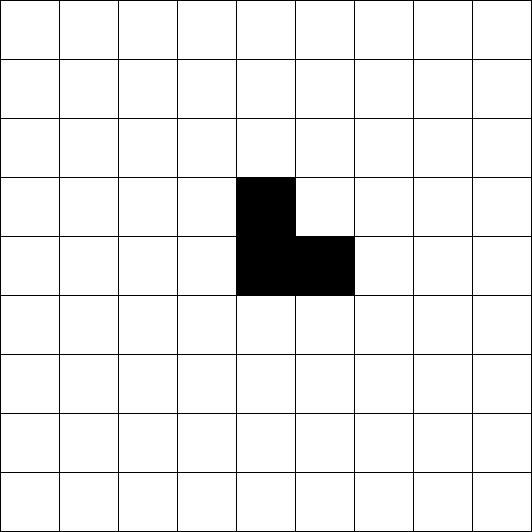
\includegraphics[width=0.19\textwidth]{chapters/nmp/images/grids/maxpdatum/delay2/maxWithPDatum_delay2_four_generations_round_1.pdf}}
    \subcaptionbox{Round 2}{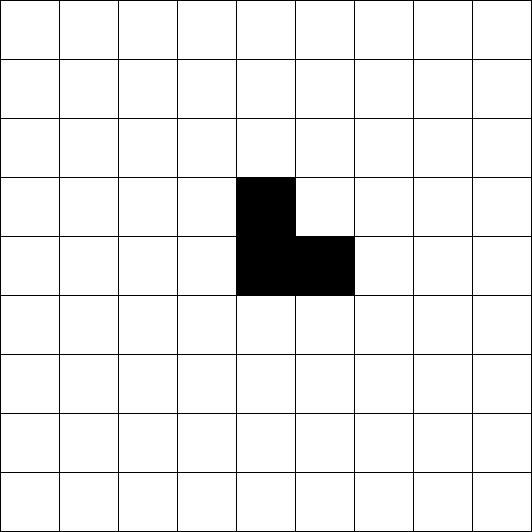
\includegraphics[width=0.19\textwidth]{chapters/nmp/images/grids/maxpdatum/delay2/maxWithPDatum_delay2_four_generations_round_2.pdf}}
    \subcaptionbox{Round 3}{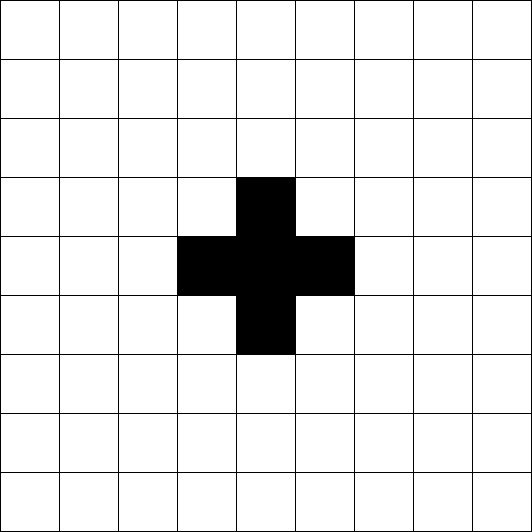
\includegraphics[width=0.19\textwidth]{chapters/nmp/images/grids/maxpdatum/delay2/maxWithPDatum_delay2_four_generations_round_3.pdf}}
    \subcaptionbox{Round 4}{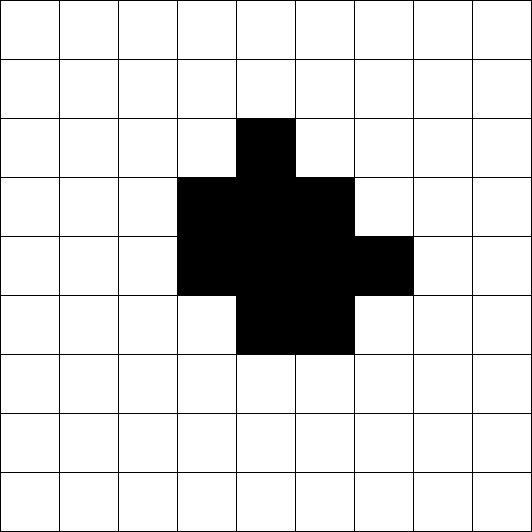
\includegraphics[width=0.19\textwidth]{chapters/nmp/images/grids/maxpdatum/delay2/maxWithPDatum_delay2_four_generations_round_4.pdf}}
    \subcaptionbox{Round 5}{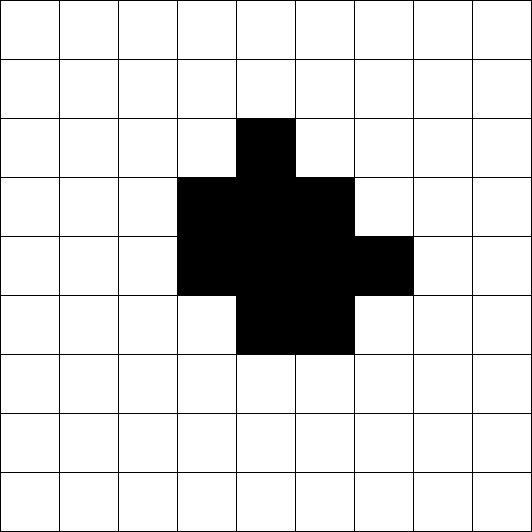
\includegraphics[width=0.19\textwidth]{chapters/nmp/images/grids/maxpdatum/delay2/maxWithPDatum_delay2_four_generations_round_5.pdf}}
    \subcaptionbox{Round 6}{
\includegraphics[width=0.19\textwidth]{chapters/nmp/images/grids/maxpdatum/delay2/maxWithPDatum_delay2_four_generations_round_6.pdf}}
    \subcaptionbox{Round 7}{
\includegraphics[width=0.19\textwidth]{chapters/nmp/images/grids/maxpdatum/delay2/maxWithPDatum_delay2_four_generations_round_7.pdf}}
    \subcaptionbox{Round 8}{
\includegraphics[width=0.19\textwidth]{chapters/nmp/images/grids/maxpdatum/delay2/maxWithPDatum_delay2_four_generations_round_8.pdf}}
    \subcaptionbox{Round 9}{
\includegraphics[width=0.19\textwidth]{chapters/nmp/images/grids/maxpdatum/delay2/maxWithPDatum_delay2_four_generations_round_9.pdf}}
    \caption[Visualisation of the spread of `influence' from the centre \glsxtrshort{pe} during \glsxtrlong{nmp}]{Visualisation of the spread of `influence' from the centre \gls{pe} during \gls{nmp}.  Each square's value was computed as the maximum over both the last messages received, and a datum stored by the \gls{pe}, and with delivery delays of two rounds on messages going to the neighbours below and to the left}
    \label{fig:nmp:maxpdatumdelays}
\end{figure}

More interesting is \cref{fig:nmp:maxpdatumdelays}.  The same update computations were performed, but a two-round delay was introduced for the delivery of messages to the neighbours below and to the left of the sending \gls{pe}.  Messages destined for the neighbours to the right and above of the sending \gls{pe} were delivered without delays, as in \cref{fig:nmp:maxpdatum}.  The eventual symmetry of the shape may seem surprising at first, but is actually logical.  Remember that every \gls{pe}/square on the grid is a neighbour of the ones to the top and right, and will only receive messages from those neighbours after the two-round delay --- which consequently means that they in turn only send out messages to their bottom and left \emph{after} that delay.  See also \cref{prop:nmp:3}.

What might happen if there is a systematic delay in only one direction, and thus potentially messages from all other neighbours might arrive relatively quickly?  This is examined in \cref{fig:nmp:maxpdatumdelayswestonly}, where a two round delay was introduced for messages sent to the left only.  In this case, the overall shape of the \glspl{pe} on the grid who have received a message containing `influence' from the centre \gls{pe} still invariably ends up returning to a symmetrical, balanced shape.  It is a different shape, however, from that seen in \cref{fig:nmp:maxpdatum,fig:nmp:maxpdatumdelays}, and is not centred on the centre \gls{pe}.  Instead, it grows with a bias towards the right.%  This eventual symmetry may appear surprising at first, but is to be expected for similar reasons to the basis for \autoref{prop:3}.  A \gls{pe} can only send a message to a neighbour once it has received the messages from the other neighbours, and this dependency is (effectively) transitive.  Thus, if some messages take much longer to arrive, \glspl{pe} will end up being forced to wait for them, directly or indirectly.

\begin{figure}
    \centering
    \subcaptionbox{Round 0}{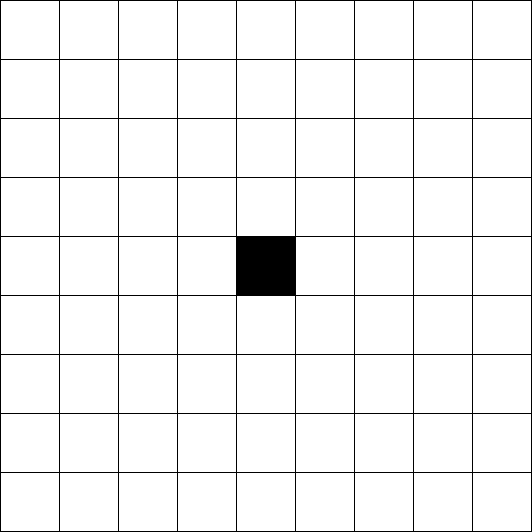
\includegraphics[width=0.19\textwidth]{chapters/nmp/images/grids/maxpdatum/delay2westonly/maxWithPDatum_delay2_west_only_four_generations_round_0.pdf}}
    \subcaptionbox{Round 1}{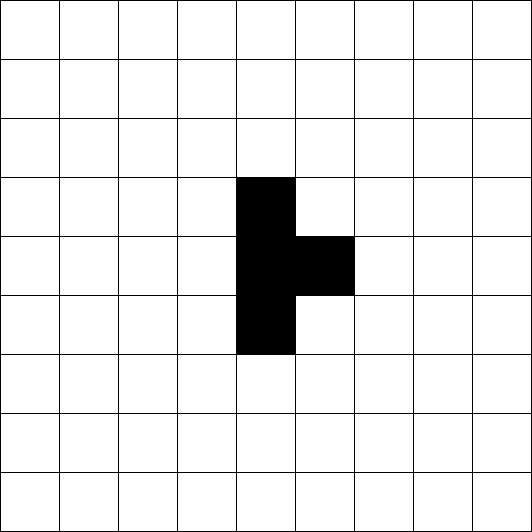
\includegraphics[width=0.19\textwidth]{chapters/nmp/images/grids/maxpdatum/delay2westonly/maxWithPDatum_delay2_west_only_four_generations_round_1.pdf}}
    \subcaptionbox{Round 2}{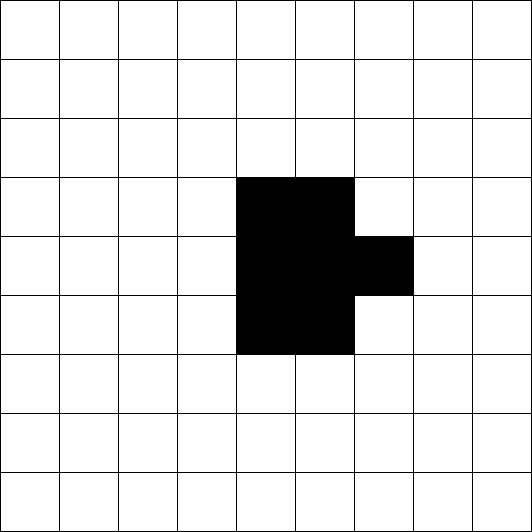
\includegraphics[width=0.19\textwidth]{chapters/nmp/images/grids/maxpdatum/delay2westonly/maxWithPDatum_delay2_west_only_four_generations_round_2.pdf}}
    \subcaptionbox{Round 3}{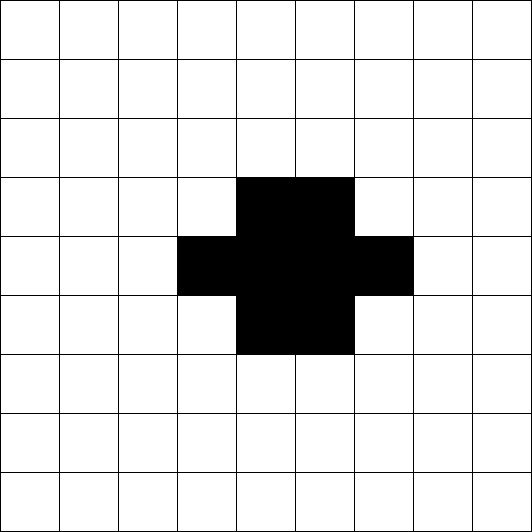
\includegraphics[width=0.19\textwidth]{chapters/nmp/images/grids/maxpdatum/delay2westonly/maxWithPDatum_delay2_west_only_four_generations_round_3.pdf}}
    \subcaptionbox{Round 4}{
\includegraphics[width=0.19\textwidth]{chapters/nmp/images/grids/maxpdatum/delay2westonly/maxWithPDatum_delay2_west_only_four_generations_round_4.pdf}}
    \subcaptionbox{Round 5}{
\includegraphics[width=0.19\textwidth]{chapters/nmp/images/grids/maxpdatum/delay2westonly/maxWithPDatum_delay2_west_only_four_generations_round_5.pdf}}
    \subcaptionbox{Round 6}{
\includegraphics[width=0.19\textwidth]{chapters/nmp/images/grids/maxpdatum/delay2westonly/maxWithPDatum_delay2_west_only_four_generations_round_6.pdf}}
    \subcaptionbox{Round 7}{
\includegraphics[width=0.19\textwidth]{chapters/nmp/images/grids/maxpdatum/delay2westonly/maxWithPDatum_delay2_west_only_four_generations_round_7.pdf}}
    \subcaptionbox{Round 8}{
\includegraphics[width=0.19\textwidth]{chapters/nmp/images/grids/maxpdatum/delay2westonly/maxWithPDatum_delay2_west_only_four_generations_round_8.pdf}}
    \subcaptionbox{Round 9}{
\includegraphics[width=0.19\textwidth]{chapters/nmp/images/grids/maxpdatum/delay2westonly/maxWithPDatum_delay2_west_only_four_generations_round_9.pdf}}
    \caption[Visualisation of the spread of `influence' from the centre \glsxtrshort{pe} during \glsxtrlong{nmp}.]{Visualisation of the spread of `influence' from the centre \gls{pe} during \gls{nmp}.  Each square's value was computed as the maximum over both the last messages received, and a datum stored by the \gls{pe}, and with delivery delays of two rounds on messages going to the left only}
    \label{fig:nmp:maxpdatumdelayswestonly}
\end{figure}

\subsubsection{Maximum over messages received}
\begin{figure}
    \centering
    \subcaptionbox{Round 0}{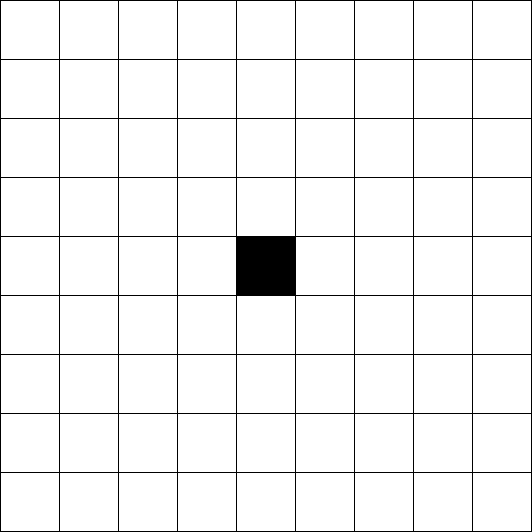
\includegraphics[width=0.19\textwidth]{chapters/nmp/images/grids/max/nodelay/max_no_delay_four_generations_round_0.pdf}}
    \subcaptionbox{Round 1}{
\includegraphics[width=0.19\textwidth]{chapters/nmp/images/grids/max/nodelay/max_no_delay_four_generations_round_1.pdf}}
    \subcaptionbox{Round 2}{
\includegraphics[width=0.19\textwidth]{chapters/nmp/images/grids/max/nodelay/max_no_delay_four_generations_round_2.pdf}}
    \subcaptionbox{Round 3}{
\includegraphics[width=0.19\textwidth]{chapters/nmp/images/grids/max/nodelay/max_no_delay_four_generations_round_3.pdf}}
    \subcaptionbox{Round 4}{
\includegraphics[width=0.19\textwidth]{chapters/nmp/images/grids/max/nodelay/max_no_delay_four_generations_round_4.pdf}}
    \caption[Visualisation of the spread of `influence' from the centre \glsxtrshort{pe} during \glsxtrlong{nmp}]{Visualisation of the spread of `influence' from the centre \gls{pe} during \gls{nmp}.  Each square's value was computed as the maximum over the last messages received}
    \label{fig:nmp:max}
\end{figure}

The sequence in \cref{fig:nmp:max} was produced by using the maximum of the messages received from the other neighbours when computing the new outgoing messages for each \gls{pe}.\footnote{Given that both systems only have two values for each cell and updates to a given cell are based on values in surrounding ones, it does not seem coincidental that this progression bears some resemblance to Conway's Game of Life.}  As with the sequence in \cref{fig:nmp:maxpdatum}, the spread of the influence from the centre \gls{pe} moves outward, similar to an expanding `+' shape.  Notably, however, points in the grid (except the centre \gls{pe} for one round) oscillate between the minimum and the maximum, showing that the influence from the centre \gls{pe} is only relevant for every second message update computation.  Felzenzswalb \& Huttenlocher \cite{Felzenszwalb2006} noticed this oscillating behaviour and used it to halve the number of computations required to produce the same results in their improved \gls{bp} \gls{sm} implementation.

\subsubsection{Mean over messages received}
\begin{figure}
    \centering
    \subcaptionbox{Round 0}{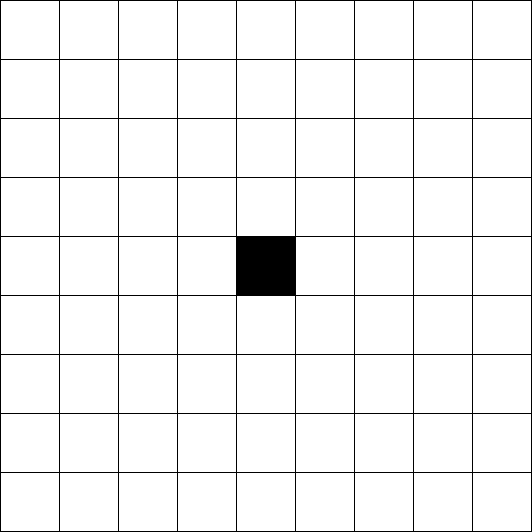
\includegraphics[width=0.19\textwidth]{chapters/nmp/images/grids/mean/nodelay/mean_no_delay_four_generations_round_0.pdf}}
    \subcaptionbox{Round 1}{
\includegraphics[width=0.19\textwidth]{chapters/nmp/images/grids/mean/nodelay/mean_no_delay_four_generations_round_1.pdf}}
    \subcaptionbox{Round 2}{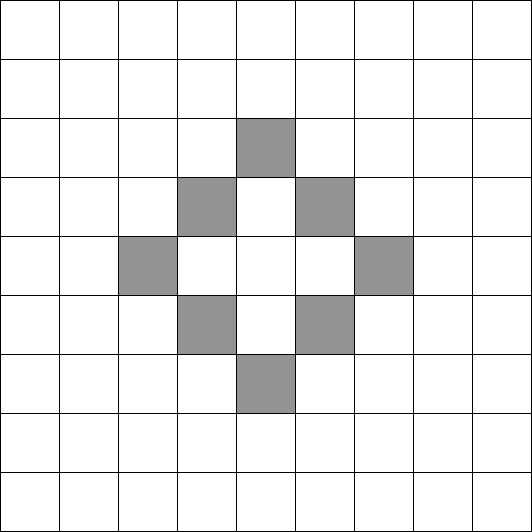
\includegraphics[width=0.19\textwidth]{chapters/nmp/images/grids/mean/nodelay/mean_no_delay_four_generations_round_2.pdf}}
    \subcaptionbox{Round 3}{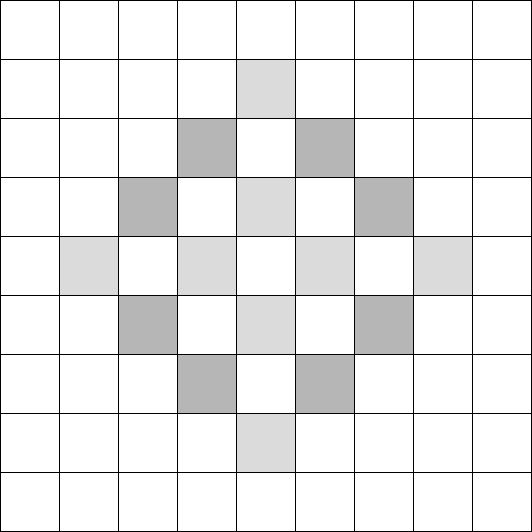
\includegraphics[width=0.19\textwidth]{chapters/nmp/images/grids/mean/nodelay/mean_no_delay_four_generations_round_3.pdf}}
    \subcaptionbox{Round 4}{
\includegraphics[width=0.19\textwidth]{chapters/nmp/images/grids/mean/nodelay/mean_no_delay_four_generations_round_4.pdf}}
    \caption[Visualisation of the spread of `influence' from the centre \glsxtrshort{pe} during \glsxtrlong{nmp}]{Visualisation of the spread of `influence' from the centre \gls{pe} during \gls{nmp}.  Each square's value was computed as the mean over the last messages received}
    \label{fig:nmp:mean}
\end{figure}

The sequence in \cref{fig:nmp:mean} was produced by using the mean of the messages received from the other neighbours when computing the new outgoing messages for each \gls{pe}.  This sequence makes it clear that as the initial information from a given \gls{pe} diffuses across the grid, its direct influence upon the data in the \glspl{pe} gradually dilutes.  After just four rounds of message passing, the `signal strength' from the centre \gls{pe} has become so weak as to be almost imperceptible in the most distant locations it has reached, \eg{} points (0,4) and (4,8), assuming a zero-based grid count beginning in the upper-left corner.